\newcommand{\dir}{../preface}

%========================= PREFACE ========================= 
\ifthenelse{\boolean{edthesis}}
 {
   \begin{prefacepart}
   \pagenumbering{roman} 
}
{
  \frontmatter
}

\thispagestyle{empty}

\begin{minipage}{\textwidth}
\end{minipage}
\begin{center}
\vspace{2cm}
{ \Huge Thesis Title \\second line of title
  \par
  \vspace{0.5cm} 
{\Large Author Name \par}
}
\vfill
\centerline{
\includegraphics[width=0.35\textwidth]{\dir/2Line2ColCMYK_CS3}}
\vspace{0.5cm}
Thesis submitted in fulfilment of\\
the requirements for the degree of\\ 
Doctor of Philosophy\\ 
to the\\
University of Edinburgh --- 20xx
\end{center}

\newpage
\thispagestyle{empty}



\chapter*{Declaration}
\vspace*{2\baselineskip}
I declare that this thesis has been composed 
solely by myself and that it has not been submitted, either in whole or
in part, in any previous application for a degree.
Except where otherwise acknowledged, the work presented is entirely my
own.
\vspace{6\baselineskip}\\
\begin{flushright}
\hspace*{\fill}
Hauke Andreas Holtkamp
\newline
\newdateformat{mydate}{\monthname[\THEMONTH] \THEYEAR}
\mydate\today
\end{flushright}


\cleardoublepage

\chapter{Abstract}
\markboth{\MakeUppercase{Abstract}}{\MakeUppercase{Abstract}}
Lorem ipsum dolor sit amet, consetetur sadipscing elitr, sed diam nonumy eirmod tempor invidunt ut labore et dolore magna aliquyam erat, sed diam voluptua. At vero eos et accusam et justo duo dolores et ea rebum. Stet clita kasd gubergren, no sea takimata sanctus est Lorem ipsum dolor sit amet. Lorem ipsum dolor sit amet, consetetur sadipscing elitr, sed diam nonumy eirmod tempor invidunt ut labore et dolore magna aliquyam erat, sed diam voluptua. At vero eos et accusam et justo duo dolores et ea rebum. Stet clita kasd gubergren, no sea takimata sanctus est Lorem ipsum dolor sit amet.
\chapter*{Acknowledgements}
\markboth{\MakeUppercase{Acknowledgements}}{\MakeUppercase{Acknowledgements}}

Thanks...

{\setlength{\parskip}{0ex plus 0.5ex minus 0.2ex}

\ifthenelse{\boolean{edthesis}}
 {
  \begin{singlespace}
 }{}

\tableofcontents
\listoftables
\listoffigures
% Glossary stuff
\chapter{List of Acronyms}
\begin{acronym}[WINNER]
 %% Definition of Acronyms. '%m% indicates that it is an acronym of minor usage

\acro{3GPP}[3GPP]{3rd Generation Partnership Project} %m
\acro{AA}[AA]{Antenna Adaptation}
\acro{AC}[AC]{Alternating Current}
\acro{ACLR}[ACLR]{Adjacent Carrier Leakage Ratio}  %m
\acro{ADC}[ADC]{Analog-to-Digital Converter}  %m
\acro{ASIC}[ASIC]{Application-Specific Integrated Circuit}  %m
\acro{ASIP}[ASIP]{Application-Specific Instruction-set Processor}  %m
\acro{BA}[BA]{Bandwidth Adaptation} 
\acro{BB}[BB]{Baseband} 
\acro{BS}[BS]{Base Station}
% \acro{CAGR}[CAGR]{Compound Annual Growth Rate}
\acro{CDM}[CDM]{Code Division Multiplexing}  %m
\acro{CDMA}[CDMA]{Code Division Multiple Access}  %m
\acro{CMOS}[CMOS]{Complementary metal–oxide–semiconductor}  %m
\acro{CSI}[CSI]{Channel State Information}
\acro{DAC}[DAC]{Digital-to-Analog Converter}  %m
\acro{DC}[DC]{Direct Current}
\acro{DTX}[DTX]{Discontinuous Transmission}
\acro{EARTH}[EARTH]{Energy Aware Radio and neTwork tecHnologies}
% \acro{EU}[EU]{European Union}
\acro{FDD}[FDD]{Frequency Division Duplex}
\acro{FDM}[FDM]{Frequency Division Multiplexing}  %m
\acro{FDMA}[FDMA]{Frequency Division Multiple Access}
\acro{FFT}[FFT]{Fast Fourier Transform}  %m
% \acro{FP}[FP]{Framework Programme}
\acro{FPGA}[FPGA]{Field-Programmable Gate Array}  %m
\acro{GOPS}[GOPS]{Giga Operations Per Second}  %m
\acro{GSM}[GSM]{Global System for Mobile communications} 
\acro{HetNet}[HetNet]{Heterogeneous Network}
\acro{ICT}[ICT]{Information and Communication Technologies}  %m
% \acro{IPOPT}[IPOPT]{Interior Point OPTimizer}
\acro{IQ}[IQ]{In-phase/Quadrature} %m
\acro{LNA}[LNA]{Low-Noise Amplifier}  %m
\acro{LTE}[LTE]{Long Term Evolution}
\acro{M2M}[M2M]{Machine-to-Machine} %m
\acro{MCS}[MCS]{Modulation and Coding Scheme} %m
\acro{MIMO}[MIMO]{Multiple-Input Multiple-Output}
\acro{OFDM}[OFDM]{Orthogonal Frequency Division Multiplexing}
\acro{OFDMA}[OFDMA]{Orthogonal Frequency Division Multiple Access}
\acro{OPEX}[OPEX]{Operating Expenses} %m
\acro{PA}[PA]{Power Amplifier}
\acro{PAPR}[PAPR]{Peak-to-Average Power Ratio} %m
\acro{PC}[PC]{Power Control}
\acro{PRAIS}[PRAIS]{Power and Resource Allocation Including Sleep}
\acro{QoE}[QoE]{Quality of Experience} %m
\acro{QoS}[QoS]{Quality of Service} %m
\acro{RAPS}[RAPS]{Resource allocation using Antenna adaptation, Power control and Sleep modes}
% \acro{RB}[RB]{Resource Block}
\acro{RF}[RF]{Radio Frequency}
\acro{RCG}[RCG]{Rate Craving Greedy}
\acro{RRH}[RRH]{Remote Radio Head} %m
\acro{RRM}[RRM]{Radio Resource Management}
% \acro{SAE}[SAE]{System Architecture Evolution}
\acro{SC-FDMA}[SC-FDMA]{Single-carrier FDMA} %m
\acro{SIMO}[SIMO]{Single-Input Multiple-Output}
\acro{SINR}[SINR]{Signal-to-Interference-and-Noise-Ratio}
\acro{SISO}[SISO]{Single-Input Single-Output}
\acro{SNR}[SNR]{Signal-to-Noise-Ratio}
\acro{SOTA}[SotA]{State-Of-The-Art}
\acro{TDD}[TDD]{Time Division Duplex} %m
\acro{TDM}[TDM]{Time Division Multiplexing}
\acro{TDMA}[TDMA]{Time Division Multiple Access}
\acro{UE}[UE]{User Equipment}
\acro{UMTS}[UMTS]{Universal Mobile Telecommunications System} %m
\acro{VCO}[VCO]{Voltage-Controlled Oscillator} %m
% \acro{WINNER}[WINNER]{Wireless world INitiative NEw Radio}
\acro{WSN}[WSN]{Wireless Sensor Network} %m

\end{acronym}


\cleardoublepage
\printnomenclature[0.6in] % requires 'makeindex ed_thesis.nlo -s nomencl.ist -o ed_thesis.nls' to update
% \renewcommand{\nomname}{List of Symbols}
% \markboth{\MakeUppercase{\nomname}}{\MakeUppercase{\nomname}}
% \addcontentsline{toc}{chapter}{List of Symbols}
%\printglossary
\ifthenelse{\boolean{edthesis}}
 {
  \end{singlespace}
 }{}
}

\ifthenelse{\boolean{edthesis}}
 {
   \end{prefacepart}
   \pagenumbering{arabic} 
}
{
   \mainmatter
}

\acresetall % reset acronyms which were used in nomenclature and abstract

%========================= CHAPTERS ========================= 
\renewcommand{\dir}{../chapter1/chapter/}
\chapter{Introduction}
\label{ch:introduction}

\section{Overview}
This chapter...

\section{Thesis Context}

Since the emergence of mobile communications...

\section{Thesis Contributions}
This thesis contributes t...

\section{Thesis Structure}
Chapter~\ref{ch:motivation} ...


\acresetall % reset acronyms which were used in nomenclature and abstract

\renewcommand{\dir}{../chapter2/chapter/}
\chapter{Motivation and Background}
\label{ch:motivation}

\section{Overview}
This chapter first...

\section{Energy Efficient Base Stations}
\label{sect:eebs}
A sample figure.

\begin{figure}
\centering
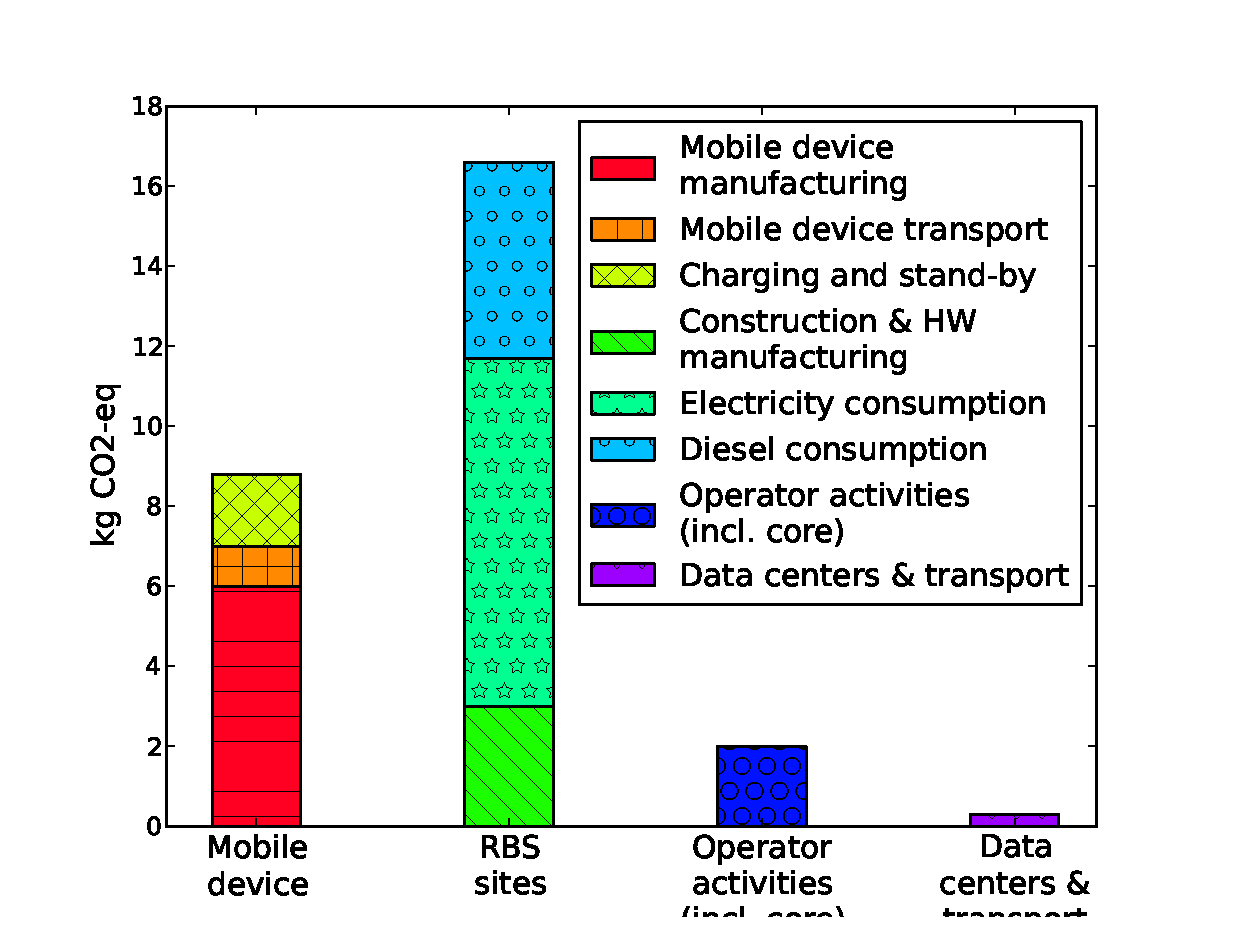
\includegraphics[width=0.6\textwidth]{\dir/img/carbonfootprint}
\caption[The carbon footprint for an average subscriber in 2007]{The carbon footprint (\coo-equivalent emissions, see Section~\ref{sect:quantEE}) for an average subscriber in 2007~\cite{mmlfl1001}.} % from enablers paper, my own. How to reference?
\label{fig:4}
\end{figure}

\section{Quantifying Energy Efficiency}
\label{sect:quantEE}
Enhancing the energy efficiency of communication networks has led to a field of research popularly labelled \emph{Green Radio}...

\section{Green Radio in Literature}
Historically, ...

\section{Technical Background}
\label{background}

The following sections outline some fundamental concepts ...

\subsection{\ac{LTE}}

\ac{LTE}~\cite{book:dps1101} is a wireless access standard superseding the \ac{GSM} and \ac{UMTS} for increased network capacities. 

\subsection{Multi-carrier Technology}
\label{sect:multicarrier}
The wireless medium is inherently shared...

\subsection{Network Simulation}

For many problems in communications research...

\section{Summary}
This chapter served to provide ...


\acresetall % reset acronyms which were used in nomenclature and abstract

\renewcommand{\dir}{../chapter3/chapter/}
\chapter{Power Saving on the Device Level}
\label{ch:device}

\section{Overview}
Power models describe ...

\section{Challenges in Power Modeling}
\label{ch3:challenges}
Generic modeling of \ac{BS} power consumption is not a trivial task for multiple reasons...

\section{Existing Power Models}
\label{ch3:existing}
In literature, three distinct power models for wireless transmitters are proposed and applied...

\section{The Component Power Model}
\label{ch3:componentmodel}
Before the description of the model, it is necessary to make some introductory remarks.

\subsection{Remarks}

First, ...

\subsection{The Components of a \ac{BS}}
The modelled \ac{LTE} macro \ac{BS} consists of ...

\subsubsection{Antenna Interface}
This passive component is ...

\subsubsection{\ac{PA}}
The \ac{PA} amplifies ...


\subsubsection{\ac{RF} Transceiver}
The \ac{RF} transceiver provides the signal conversion ...

\subsubsection{\ac{BB} Unit}
The \ac{BB} unit generates ...


\subsubsection{\ac{DC}-\ac{DC}-Conversion}
To supply the required \ac{DC} voltages ...

\subsubsection{Mains Supply/\ac{AC}-\ac{DC}-Conversion}
Power from the the \ac{AC} mains grid is converted to \ac{DC} by the mains power supply unit...

\subsubsection{Cooling}
Macro \acp{BS} are typically housed in a cooled cabinet...

\subsection{\ac{BS} Power Consumption}
The power consumption...

\section{The Parameterized Power Model}
\label{parameterizedmodel}
The power model described above is ...

\begin{table*}[t]
\centering
\begin{tabular}{|c|c|c|c|c|c|c|c|c|c|}
\hline
 $P_{\mathrm{PA,limit}}$	& $\eta_\mathrm{PA,max}$	& $\theta$	& $P_\mathrm{BB}$	& $P_\mathrm{RF}$	& $\sigma_\mathrm{feed}$	& $\sigma_\mathrm{DC}$	& $\sigma_\mathrm{COOL}$	& $\sigma_\mathrm{AC}$ 	& $M_{\mathrm{Sec}}$ 	\\
 /W			&				&		&	/W		&	/W		&				&			&	&&\\
\hline
 	80.00		& 	0.36			& 	0.15	& 	29.4		& 	12.9		& 	0.5			& 	0.075		& 	0.1
& 	0.09	& 	3			\\
\hline
\end{tabular}
\\
\begin{tabular}{|c|c|c|c|}
\hline
 $P_{\mathrm{max}}$  	& $P_{1}$  		& $\Delta_{\mathrm{p}}$ & $P_{\mathrm{S},0}$\\
		/W		&	/W		& *10\,MHz		& /W\\
\hline
	40.00		& 	460.4 		& 	4.2 		&	324.0 \\
\hline
\end{tabular}

\caption[Parameter breakdown]{Parameter breakdown.}
\label{tab:powerbreakdownmaximumload}
\end{table*}

\section{The Affine Power Model}
\label{affinemodel}
In preparation for the following chapters of this thesis...

\section{Summary}
\label{ch3:summary}
In this chapter, ...

\acresetall % reset acronyms which were used in nomenclature and abstract

\renewcommand{\dir}{../chapter4/chapter/}
\chapter{Power Saving on the Cell Level}
\label{ch:cell}

\section{Overview}
As introduced in Chapter~\ref{ch:motivation}...

\section{Power-saving \ac{RRM} in Literature}
\label{ch4:literature}
In literature, ...

\section{\ac{PC} and \acs{TDMA}}
\label{ch4:pctdma}

When the number of bits transmitted ...

Equation example
\begin{equation}
  A + B = C
 \label{eq:OP}
\end{equation}

Subequation example
\begin{subequations}
\begin{align}
& \underset{\mu, \nu}{\text{minimize}} 		& 	P_{\mathrm{supply}}(\overline{R}_k) 	&=  \left[ \sum_{k=1}^{K} \mu_k \left( P_0 + \Delta_{\mathrm{p}} \frac{P_{\mathrm{N}}}{G_k} \left( 2^\frac{\overline{R}_k}{W \mu_k} - 1 \right) \right) \right] + \nu P_{\mathrm{S}} \\
& \text{subject to} 				& 	 \sum_{k=1}^{K} \mu_k + \nu &= 1 \,,\label{eq:OPnumu} \\
& 						&	\nu 						&\ge 0,\label{eq:OPnu}\\
&						&	\mu_k 						&\ge 0 \quad \forall\,k, \label{eq:OPmu}\\
&						&	 0 \leq P_k 					&= \frac{P_{\mathrm{N}}}{G_k} \left( 2^{\frac{\overline{R}_k}{W \mu_k}} - 1 \right) \leq P_{\mathrm{max}} \quad \forall\,k.\label{eq:OPpmax}%
\end{align}%
\label{eq:OPJSAC}%
\end{subequations}%


\subsubsection{Power allocation on the link level}
It follows a derivation of ...

\subsubsection{Power allocation on the cell level}
Next, an optimization problem is proposed which ...

\subsubsection{Evaluation}
Next, the affine power model is taken into account...

\section{\ac{PRAIS}}
\label{ch4:PRAIS}

This section introduces the ...

\subsubsection{Joint \ac{PC} and \ac{DTX}}
When employing \ac{DTX} individually ...

\subsubsection{Problem formulation}
This section proceeds to ...

\subsubsection{Evaluation}
For the numerical analysis, ...

\section{\acf{RAPS}}
\label{ch4:RAPS}
To extend the previous analytical work ...

\subsection{Problem Formulation}
The global problem statement ...

\subsubsection{Complexity}
Dynamic subcarrier allocation ...

\subsection{Step~1: \ac{AA}, \ac{DTX} and Resource Allocation}
\label{step1}
...

\subsection{Step~2: Subcarrier and Power Allocation}
\label{step2}
This section ...

\subsection{Results}
\label{results}

...


\subsubsection{Benchmarks}
The following transmission strategies are evaluated ...

\subsubsection{Performance Analysis}
The channel value selection in ...

\section{Summary}
\label{ch4:summary}
Starting with the Shannon limit, ...
\acresetall % reset acronyms which were used in nomenclature and abstract

\renewcommand{\dir}{../chapter5/chapter/}
\chapter{Power Saving on the Network Level}
\label{ch:network}

\section{Overview}
Chapter~\ref{ch:cell} proposed ...

\section{Channel Allocation in Literature}
\label{ch5:literature}
Generally, ...

\section{System Model and Problem Formulation}
\label{ch5:problem}
The network is considered as follows...

\section{\ac{DTX} Alignment Strategies}
\label{ch5:solutions}
In this section, ...
\subsection{Sequential Alignment}
In \emph{sequential alignment}, ...


\subsection{Random Alignment}
\emph{Random alignment} ...
\subsection{P-persistent Ranking}
The synchronous alignment of uncoordinated \acp{BS} can lead to instabilities...

\subsection{Distributed \ac{DTX} Alignment with Memory}
Sample algorithm 

\begin{algorithm}
\caption{Distributed DTX alignment with memory}
\label{ch5alg1}
\begin{algorithmic}[1]
\ENSURE {$\psi, \Upsilon_{\mathrm{u}}$}
\STATE $Q \leftarrow $sort-desc-by-capacity$(\Upsilon)$
\FORALL{$\upsilon$ in $\Upsilon_{\mathrm{u}}$}
  \IF {$\psi (\upsilon) < \psi_{\mathrm{ul}}$}
    \STATE $\psi(\upsilon) \leftarrow \psi(\upsilon) + 1$
  \ENDIF
\ENDFOR
\FORALL{$\upsilon$ in $\Upsilon_{\mathrm{uu}} \backslash \{Q_0\}$}
  \IF {$\psi (\upsilon) > \psi_{\mathrm{ll}}$}
    \STATE $\psi(\upsilon) \leftarrow \psi(\upsilon) - 1$
  \ENDIF
\ENDFOR
\STATE $\psi (Q_0) \leftarrow \psi(Q_0) + 1$
\STATE $V \leftarrow $ sort-desc-by-score$(Q, \psi, \Upsilon)$
\RETURN $\psi, V, \Upsilon_{\mathrm{u}}$
\end{algorithmic}
\end{algorithm}
\nomenclature{$\psi$}{Scoring map, assigning scores to users}
\nomenclature{$\Upsilon_{\mathrm{u}}, \Upsilon_{\mathrm{uu}}$}{Set of used/unused time slots, respectively}
\nomenclature{$Q$}{Ranking tuple, time slots in order of capacity}
\nomenclature{$\psi_{\mathrm{ul}}, \psi_{\mathrm{ll}}$}{Upper/lower limit of score, respectively}
\nomenclature{$Q_0$}{Time slot with highest virtual capacity}
\nomenclature{$V$}{Priority tuple, time slots in order of score}

\section{Results}
\label{ch5:results}
This section ...
\subsubsection{Simulation Environment and Resource Block Scheduling}
The four strategies were tested ...
\subsubsection{Power Consumption}
To assess ...

\subsubsection{Convergence}
Another relevant aspect is ...

\subsubsection{Reliability}
An important aspect ...

\subsubsection{Complexity}
With regard to complexity...
\subsubsection{Interpretation}
...

\section{Summary}
\label{ch5:summary}
In this chapter, ...

\acresetall % reset acronyms which were used in nomenclature and abstract

\renewcommand{\dir}{../chapter6/chapter/}
\chapter{Conclusions, Limitations and Future Work}
\label{ch:conclusion}

\section{Summary and Conclusions}
In this thesis, ...

\section{Limitations and Future Work}
The most important limitation to the techniques proposed in this thesis ...

%========================= Appendix ========================= 
\renewcommand{\chaptermark}[1]{%
 \markboth{\MakeUppercase{%
 \appendixname} \ \thechapter.%
 \ #1}{}}
\renewcommand{\dir}{../appendix/appendix}
\begin{appendices}
% \chapter{Selected Publications}
% This chapter contains work either already published or under submission.

% Publication list:
% \begin{enumerate}
%  \item Enablers for Energy Efficiency Wireless Networks (VTC-Fall 2010)~\cite{aghimfbhz1001_own}
%  \item Fundamental Limits of Energy-Efficient Resource Sharing, Power Control and Discontinuous Transmission (FNMS 2011)~\cite{ha1101_own}
%  \item Minimal Average Consumption Downlink Base Station Power Control Strategy (pimrc 2011)~\cite{hah1101a_own}
%  \item On Minimizing Base Station Power Consumption (VTC-Fall 2011)~\cite{hah1101_own}
%  \item Green Communications: Theoretical Fundamentals, Algorithms and Applications (CRC Press, Sep 2012)~\cite{wrz1201_own} %http://www.amazon.com/Green-Communications-Theoretical-Fundamentals-Applications/dp/1466501073/ref=sr_1_1?ie=UTF8&qid=1349753032&sr=8-1&keywords=Green+Communications%3A+Theoretical+Fundamentals
%  \item Minimizing Base Station Power Consumption (JSAC-SI SEED, Dec 2014)~\cite{habh1301_own}
%  \item Flexible power modeling of LTE base stations (WCNC 2012)~\cite{ddgfahwsr1201_own}
%  \item Distributed DTX Alignment with Memory (submitted to pimrc 2013)~\cite{hdh1301_own}
%  \item OFDMA Basestation Power-saving Via Joint Power Control and DTX in Cellular Systems (submitted to VTC-Fall 2013)~\cite{hh1301_own}
%  \item A Parameterized Base Station Power Model (submitted to Communications Letters in 2013)~\cite{hag1301_own}
% \end{enumerate}

\chapter{Appendix} % * prevents appearance in ToC

\section{Proof of Convexity for Problem~\eqref{eq:OP}}
\label{appendix:proof1}
This proof shows that ...

\section{Proof of Convexity for Problem~\eqref{eq:OPJSAC}}
\label{appendix:proof2}
This proof shows that...

\chapter{List of Publications}
This chapter contains a list of publications related to this thesis ordered by academic publication status (published, accepted, submitted) and other type (project reports and book contributions).

\section{Published}
\begin{itemize}
 \item Gunther Auer and Istv\'an G\'odor and L\'aszl\'o H\'evizi and Muhammad Ali Imran and Jens Malmodin and P\'eter Fasekas and Gergely Bicz\'ok and \textbf{Hauke Holtkamp} and Dietrich Zeller and Oliver Blume and Rahim Tafazolli, {``Enablers for Energy Efficient Wireless Networks''}, \emph{Proceedings of the IEEE Vehicular Technology Conference (VTC) Fall-2010}, 2010~\cite{aghimfbhz1001_own}
 \item \textbf{Hauke Holtkamp} and Gunther Auer, {``Fundamental Limits of Energy-Efficient Resource Sharing, Power Control and Discontinuous Transmission''}, \emph{Proceedings of the Future Network \& Mobile Summit 2011}, 2011~\cite{ha1101_own}
 \item \textbf{Hauke Holtkamp} and Gunther Auer and Harald Haas, {``{Minimal Average Consumption Downlink Base Station Power Control Strategy}''}, \emph{Proceedings of the 2011 IEEE 22nd International Symposium on Personal Indoor and Mobile Radio Communications (PIMRC)}, 2011~\cite{hah1101a_own}
 \item \textbf{Hauke Holtkamp} and Gunther Auer and Harald Haas, {``{On Minimizing Base Station Power Consumption}''}, \emph{Proceedings of the Vehicular Technology Conference (VTC) Fall-2011}, 2011~\cite{hah1101_own}
 \item Claude Desset and Bj\"{o}rn Debaillie and Vito Giannini and Albrecht Fehske and Gunther Auer and \textbf{Hauke Holtkamp} and Wieslawa Wajda and Dario Sabella and Fred Richter and Manuel Gonzalez and Henrik Klessig and Istv\'an G\'odor and Per Skillermark and Magnus Olsson and Muhammad Ali Imran and Anton Ambrosy and Oliver Blume, {``{Flexible Power Modeling of LTE Base Stations}''}, \emph{Proceedings of the 2012 IEEE Wireless Communications and Networking Conference:}, 2012~\cite{ddgfahwsr1201_own}
 \item \textbf{Hauke Holtkamp} and Gunther Auer and Samer Bazzi and Harald Haas, {``{Minimizing Base Station Power Consumption}''}, \emph{IEEE Journal on Selected Areas in Communications}, 2014~\cite{habh1301_own}
\end{itemize}

\section{Accepted}
\begin{itemize}
  \item \textbf{Hauke Holtkamp} and Gunther Auer and Vito Giannini and Harald Haas, {``{A Parameterized Base Station Power Model}''}, \emph{IEEE Communications Letters}, 2013~\cite{hag1301_own}
 \item \textbf{Hauke Holtkamp} and Harald Haas, {``{OFDMA Base Station Power-saving Via Joint Power Control and DTX in Cellular Systems}''}, \emph{Proceedings of the Vehicular Technology Conference (VTC) Fall-2013}, 2013~\cite{hh1301_own}
\end{itemize}

\section{Submitted}
\begin{itemize}
 \item \textbf{Hauke Holtkamp} and Guido Dietl and Harald Haas, {``{Distributed DTX Alignment with Memory}''}, \emph{Proceedings of the 2014 IEEE International Conference on Communications (ICC)}, 2014~\cite{hdh1301_own}
\end{itemize}

\section{Project Reports}
\begin{itemize}
\item {EARTH Project Work Package 2}, {``{Deliverable D2.2: Reference Systems and Scenarios}''}, 2012~\cite{std:earthd22_own}
 \item {EARTH Project Work Package 3}, {``{Deliverable D3.3: Green Network Technologies}''}, 2012~\cite{std:earthd33_own}
\end{itemize}

\section{Contributions}
\begin{itemize}
 \item Jinsong Wu and Sundeep Rangan and Honggang Zhang, {``{Green Communications: Theoretical Fundamentals, Algorithms and Applications}''}, \emph{Taylor \& Francis Group}, 2012~\cite{wrz1201_own}
\end{itemize}


\chapter{Attached Publications}
This chapter contains all work either published or submitted for publication to academic conferences or journals. For brevity, \ac{EARTH} project deliverables~\cite{std:earthd33_own, std:earthd22_own} and a book chapter~\cite{wrz1201_own} are not listed here.
% \includepdf[pages=-,frame,scale=0.85,pagecommand={\pagestyle{plain}}]{\dir/../../attachments/vtcf10.pdf}
% \includepdf[pages=-,frame,scale=0.85,pagecommand={\pagestyle{plain}}]{\dir/../../attachments/pimrc11.pdf}
% \includepdf[pages=-,frame,scale=0.78,pagecommand={\pagestyle{plain}}]{\dir/../../attachments/fnms11.pdf}
% \includepdf[pages=-,frame,scale=0.85,pagecommand={\pagestyle{plain}}]{\dir/../../attachments/vtcf11.pdf}
% \includepdf[pages=-,frame,scale=0.78,pagecommand={\pagestyle{plain}}]{\dir/../../attachments/wcnc12.pdf}
% \includepdf[pages=-]{\dir/../../attachments/EARTH_D2.2.pdf}
% \includepdf[pages=-]{\dir/../../attachments/EARTH_D3.3.pdf}
% \includepdf[pages=-,frame,scale=0.85,pagecommand={\pagestyle{plain}}]{\dir/../../attachments/jsac13.pdf}
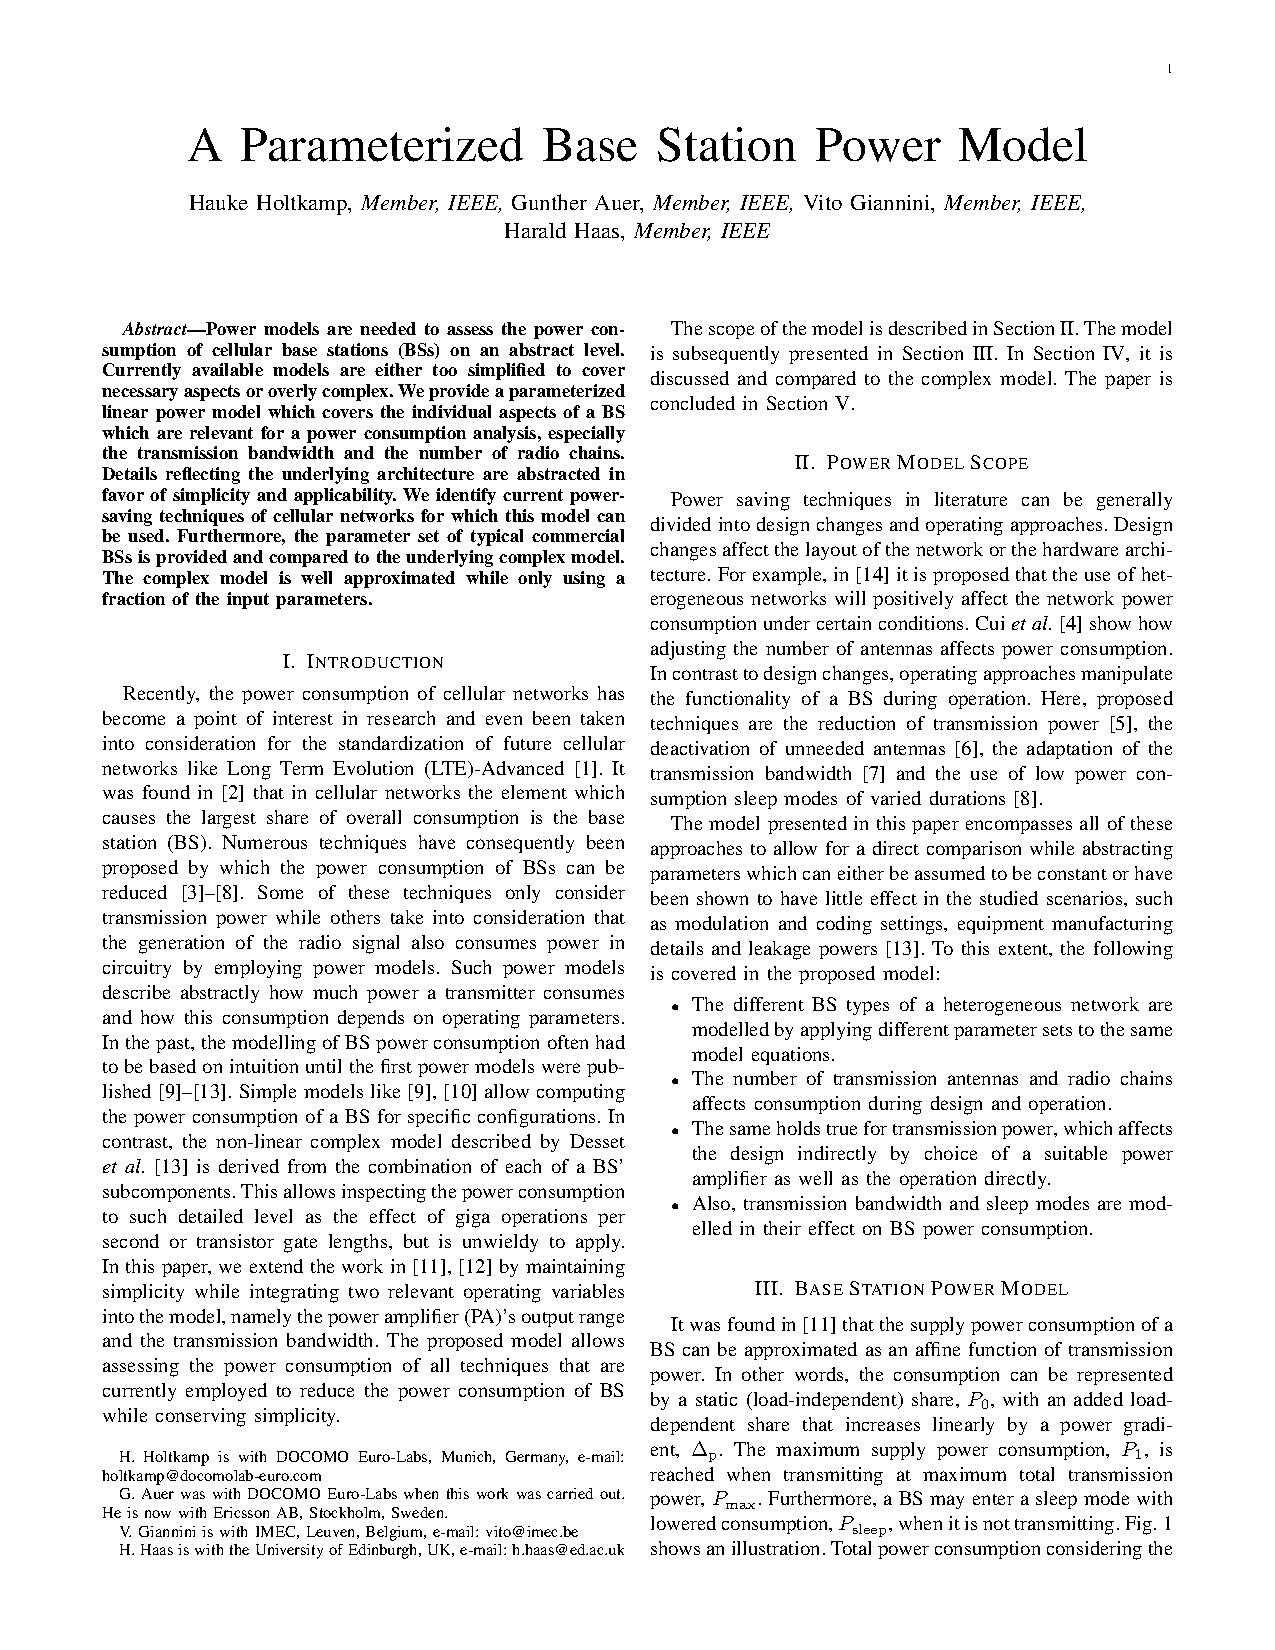
\includepdf[pages=-,frame,scale=0.85,pagecommand={\pagestyle{plain}}]{\dir/../../attachments/cl13.pdf}
% \includepdf[pages=-,frame,scale=0.85,pagecommand={\pagestyle{plain}}]{\dir/../../attachments/icc14.pdf}
% \includepdf[pages=-,frame,scale=0.85,pagecommand={\pagestyle{plain}}]{\dir/../../attachments/vtcf13.pdf}
% \includepdf[pages=-]{\dir/../../attachments/crc13.pdf}

\end{appendices}

%========================= BIBLIOGRAPHY ========================= 
\ifthenelse{\boolean{edthesis}}
 {
 \begin{singlespace}
}
{
  \backmatter
}

\nociteown{aghimfbhz1001_own,ha1101_own,hah1101a_own,hah1101_own,wrz1201_own,habh1301_own,ddgfahwsr1201_own,hdh1301_own,hh1301_own,hag1301_own, std:earthd33_own, std:earthd22_own} % may help to separate own publications from references
% own bibliography
\bibliographyown{own} % own.bib contains only my references with unique keys. Requires manual call to 'bibtex own.aux'.
\bibliographystyleown{alphayr}

\def\bibname{Literature References}
%\tocotherhead{References}
%\addcontentsline{toc}{chapter}{References}

% general bibliography
\bibliography{general,DOCOMO}
\ifthenelse{\boolean{edthesis}}
 {
  \end{singlespace}
 }{}

